  \section{Interface de Comunicação}

    \subsection{Diagrama de Classe}
      \begin{figure}[H]
        \centering
        \flushleft
  \begin{tikzpicture} 
    \begin{umlsystem}[x=0, fill=red!10]{Interface de Comunicação} 
      \umlactor[x=-5, y=-3]{Controle IF} 
      \umlactor[x=4, y=-5]{Controle}

      \umlusecase[name=lefunc]{Lê operação}
      \umlusecase[y=-2, name=leoperandos]{Lê operandos} 
      % \umlusecase[y=-4, name=saida,width=1.5cm]{Controla saída}
      \umlusecase[y=-4, name=operacao,width=1.5cm]{Envia operação} 
      \umlusecase[y=-6, name=operandos,width=1.5cm]{Envia operandos}

      \umlassoc{Controle IF}{lefunc}
      \umlassoc{Controle IF}{leoperandos}
      % \umlassoc{Controle IF}{saida}
      \umlassoc{Controle IF}{operacao}
      \umlassoc{Controle IF}{operandos}
      \umlassoc{operacao}{Controle}
      \umlassoc{operandos}{Controle}

    \end{umlsystem} 
  \end{tikzpicture}
      \end{figure}

    \subsection{Definições de Entrada e Saída}
      \FloatBarrier
      \begin{center}
        \begin{longtable}[pos]{| l | c | c | m{7cm} |} \hline         
          \multicolumn{1}{|c|}{\cellcolor[gray]{0.9}\textbf{Nome}} & 
          \multicolumn{1}{c|}{\cellcolor[gray]{0.9}\textbf{Tamanho}} & 
          \multicolumn{1}{c|}{\cellcolor[gray]{0.9}\textbf{Direção}} &
          \multicolumn{1}{c|}{\cellcolor[gray]{0.9}\textbf{Descrição}} \\ \hline
          \endfirsthead
          \hline
          \multicolumn{4}{|l|}%
          {{\bfseries continuação da página anterior}} \\
          \hline
          \multicolumn{1}{|c|}{\cellcolor[gray]{0.9}\textbf{Nome}} & 
          \multicolumn{1}{c|}{\cellcolor[gray]{0.9}\textbf{Tamanho}} & 
          \multicolumn{1}{c|}{\cellcolor[gray]{0.9}\textbf{Direção}} &
          \multicolumn{1}{c|}{\cellcolor[gray]{0.9}\textbf{Descrição}} \\ \hline
          \endhead

          \multicolumn{4}{|r|}{{continua na próxima página}} \\ \hline
          \endfoot

          \hline
          \endlastfoot

          clock\_in                & 1   & entrada   & Clock principal do sistema.    \\ \hline
          reset\_in                & 1   & entrada   & Sinal de reset geral do sistema.    \\ \hline
          rx\_data\_ready\_in      & 1   & entrada   & Indica que o dado foi recebido pelo controle RS232.    \\ \hline
          rx\_data\_in             & 8   & entrada   & Dado proveniente da transmissão.    \\ \hline
          data\_a\_out             & 8   & saída   & Dado do primeiro operando.    \\ \hline
          data\_b\_out             & 8   & saída   & Dado do segundo operando.    \\ \hline
          operation\_out          & TBD   & saída   & Código da operação.    \\ 
        \end{longtable}
      \end{center}    

    %\subsection{Datapath Interno}

    \subsection{Máquina de Estados}
      \begin{figure}[H]
        \centering
        \begin{tikzpicture} 
        \umlstateinitial[name=idle]
        \umlstatefinal[x=8, y=-3.2, name=final]
        \umlbasicstate[x=0, y=-4, do=counter++, name=read]{read\_data}  
        \umlbasicstate[x=4, y=-3.5, name=send]{send\_data}    

        \umltrans[arg={rx\_data\_ready\_in}]{idle}{read}
        \umltrans{read}{send}
        \umltrans{send}{final}
        \umltrans[recursive=-160|-120|3cm, recursive direction=right to bottom, arg={counter != 3}, pos=1.5]{read}{read} 
        \end{tikzpicture}    
      \end{figure}

    \begin{landscape}
      \subsection{Diagrama de Temporização}
        \begin{figure}[H]
          \centering
          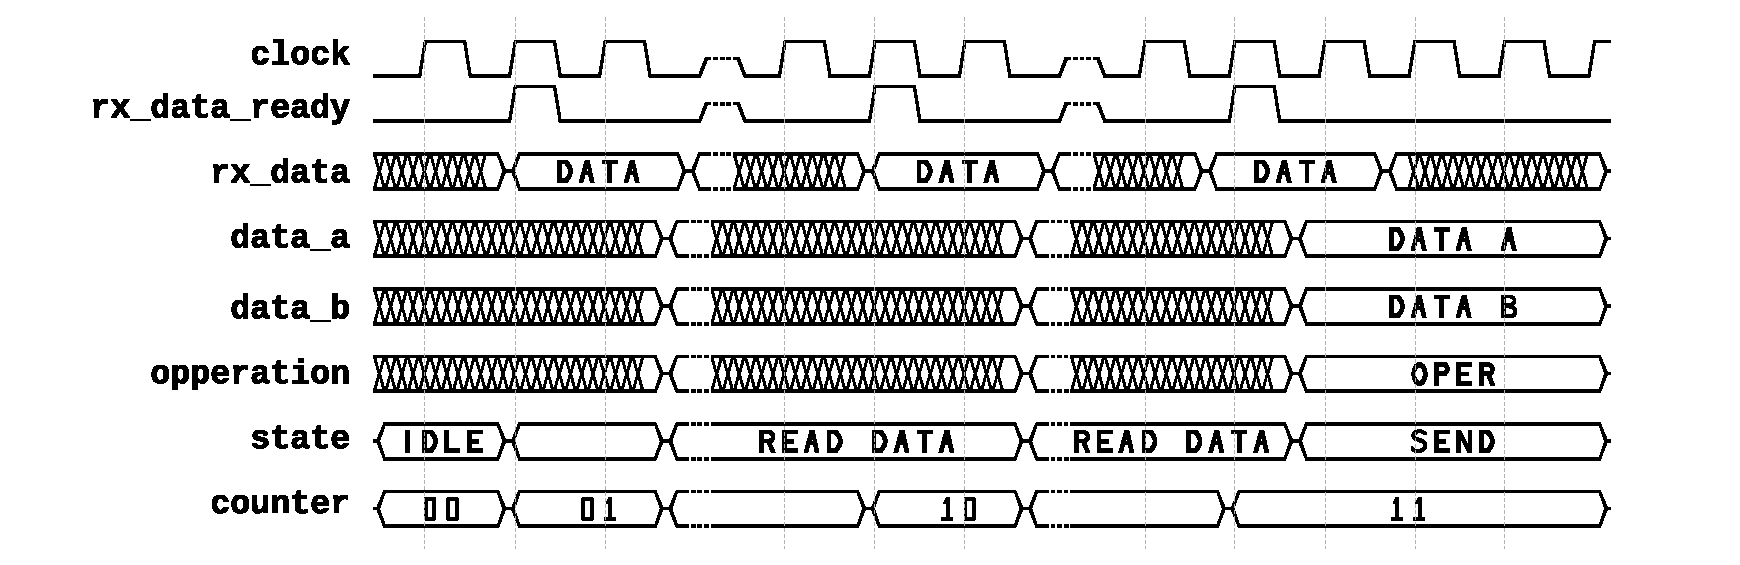
\includegraphics[width=\linewidth]{timing/comunication_timing.eps}
        \end{figure}
    \end{landscape}